\chapter{Combine Individual Modules in Simulation}

\paragraph*{}
This chapter summarizes the procedures for modularization of two functionalities: object detection and communication. Together with how the programs are tested in Webots, our goal is to have a single-world simulation with these two operating simultaneously as Python packages.

\paragraph*{}
Before all else, some changes in the communication module need to be mentioned. Initially, the consensus functionality is implemented in the communication simulation. Then a priority queue is added to support error handling when multiple robots detect objects at the same time.

\paragraph*{}
Integration of modules begins with code refactoring. At first, all of the functionalities are run independently in their own script. Now, we have developed a Python package that allows a single Webots controller to handle multiple functionalities. In Figure \ref{fig:integration}, a simple communication protocol is tested along with object detection module.

\begin{figure}[H]
    \centering
    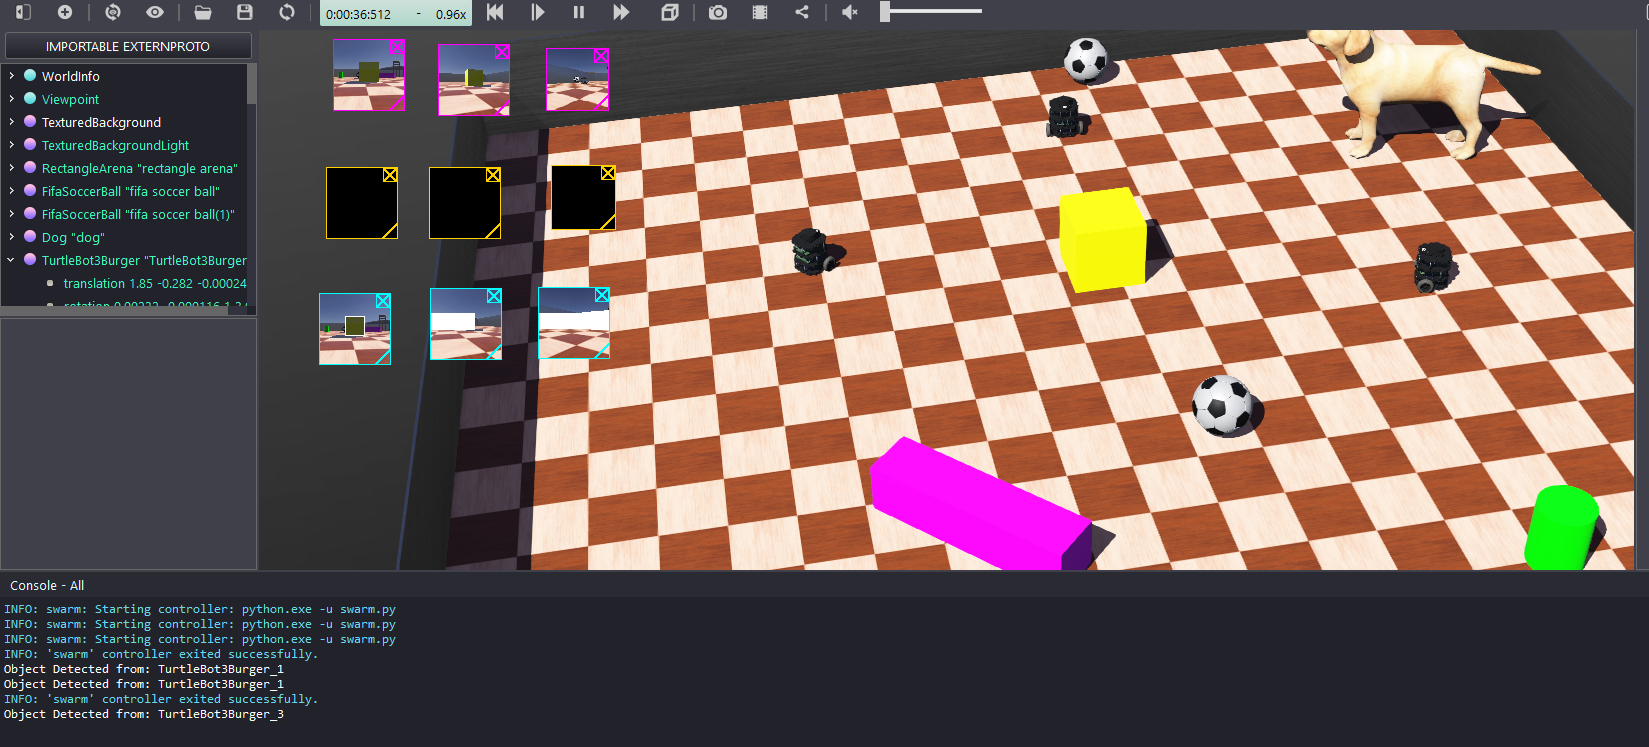
\includegraphics[width=0.8\linewidth]{assets/images/integration/swarm-com.png}
    \caption{Simulation Integration}
    \label{fig:integration}
\end{figure}

\paragraph*{}
Our next step expects to integrate the full communication protocol and equip the robots with localization, or SLAM if possible.